\section{Task 2}\label{sec:task2}

The goal of the second task is to implement a software to quantify global differences between ensembles of a PED and, from them, identify the variance level along the sequence. The input of this task are files containing the features of one PED ensemble generated during Task 1.

\subsection{Ensembles features}
Relationships between different ensembles will be identified considering the structural features of a single ensemble using the features file of task 1.

At the beginning, the software extracts the features for each ensemble (multiple conformations):
\begin{itemize}
\item Radius of gyration of each model in the ensemble. It may happen that the number of the values returned are less then the number of the ensemble's conformations, then we check on the array dimension and, if needed, a zero-padding is added.
\item Secondary structure entropy for each position across ensemble conformations exploiting its probabilistic definition between each model. 
\item Median ASA for each position across ensemble's conformations. We extract the ASA vector for each position and then we compute the median of this vector. 
\item Median RMSD using rotate-translation matrices for each conformation.
\item Median distance of each pair of equivalent positions. We consider the columns of conformation distance matrices and we return their median values.
\item Standard deviation of the distances for each position across all the ensemble's conformations.
\end{itemize}


\subsection{Global metric}
The global metric evaluates the distance between ensemble pairs. It takes into account the different nature of the features evaluated.
This metric returns the sum of partial distances for each feature:
\begin{itemize}
\item The absolute value of the difference between the mean radius of gyration for the two ensembles.
\item The Chebyshev distance between the entropies of the two ensembles. It finds the distance as the greatest of their differences along any coordinate dimension.
\item The Euclidean distance between the median ASA of the two ensembles.
\item The Euclidean distance between the median RMSD of the two ensembles.
\item The complementary of the correlation between the median distance of the two ensembles.
\end{itemize}


Using the global metric just described, the software displays the distances between two ensembles through:
\begin{itemize}
\item Heatmap: it calculates the matrix of the distances between the features of the ensembles and then builds and displays the heatmap. The distance between ensembles is highlighted with different colors based on the similarity scale reported on the right. 
\item Dendrogram: using a linkage matrix and the presented global metric, the dendrogram built combining the most similar ensembles with respect to the calculated features (with a \emph{complete} approach) is plot.
\end{itemize}

In figures \ref{heatmap} and \ref{dendrogram}, it is possible to visualize respectively the distance and similarity between the five ensembles. It can be observed that .....

\begin{figure}[H]
	\begin{minipage}[b]{0.93\textwidth}
		\centering
		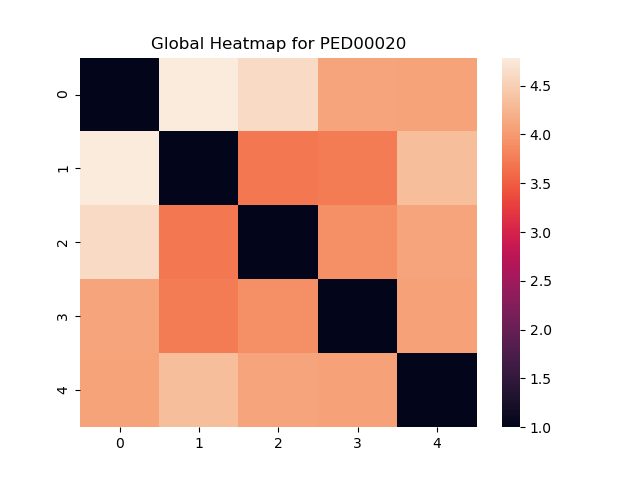
\includegraphics[width=\textwidth]{PED00020_heatmap.png}
		\caption{Heatmap of all the models.}
		\label{heatmap}
	\end{minipage}
\end{figure}
\begin{figure}[H]
	\begin{minipage}[b]{0.93\textwidth}
		\centering
		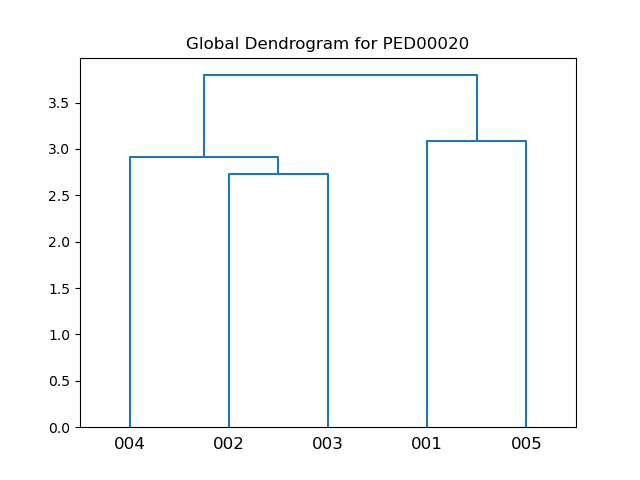
\includegraphics[width=\textwidth]{PED00020_dendrogram.png}
		\caption{Dendrogram of all the models.}
		\label{dendrogram}
	\end{minipage}
\end{figure}


\subsection{Local metric}
The local metric evaluates the variability of all the features for each position in the ensemble.
In order to compute the local variability, it considers the neighbors of the residue under analysis thanks to a window of size nine to the left and to the right of the current position.
This metric computes the mean of total values with respect each ensemble feature: 

\begin{itemize}
\item Total entropy: it considers the standard deviation among conformations entropy for each position, then it computes the mean of these values inside the window around each residual.
\item Total median ASA: it calculates the standard deviation among conformations accessible surface area for each residue, then it computes the mean of these values inside the window around the current residual.
\item Total median RMSD: it computes the standard deviation among conformations RMSD for each residue, then it calculates the mean of these values inside the window around the current residual.
\item Total standard deviation of distance: it is the trimmed mean of the standard deviation of conformations distances for each position. 
The use of a trimmed mean helps to eliminate the influence of outliers or data points on the tails on the traditional mean. Then it takes the mean of these values with respect to the window around each residual.
\end{itemize}

\begin{figure}[H]
	\begin{minipage}[b]{0.97\textwidth}
		\centering
		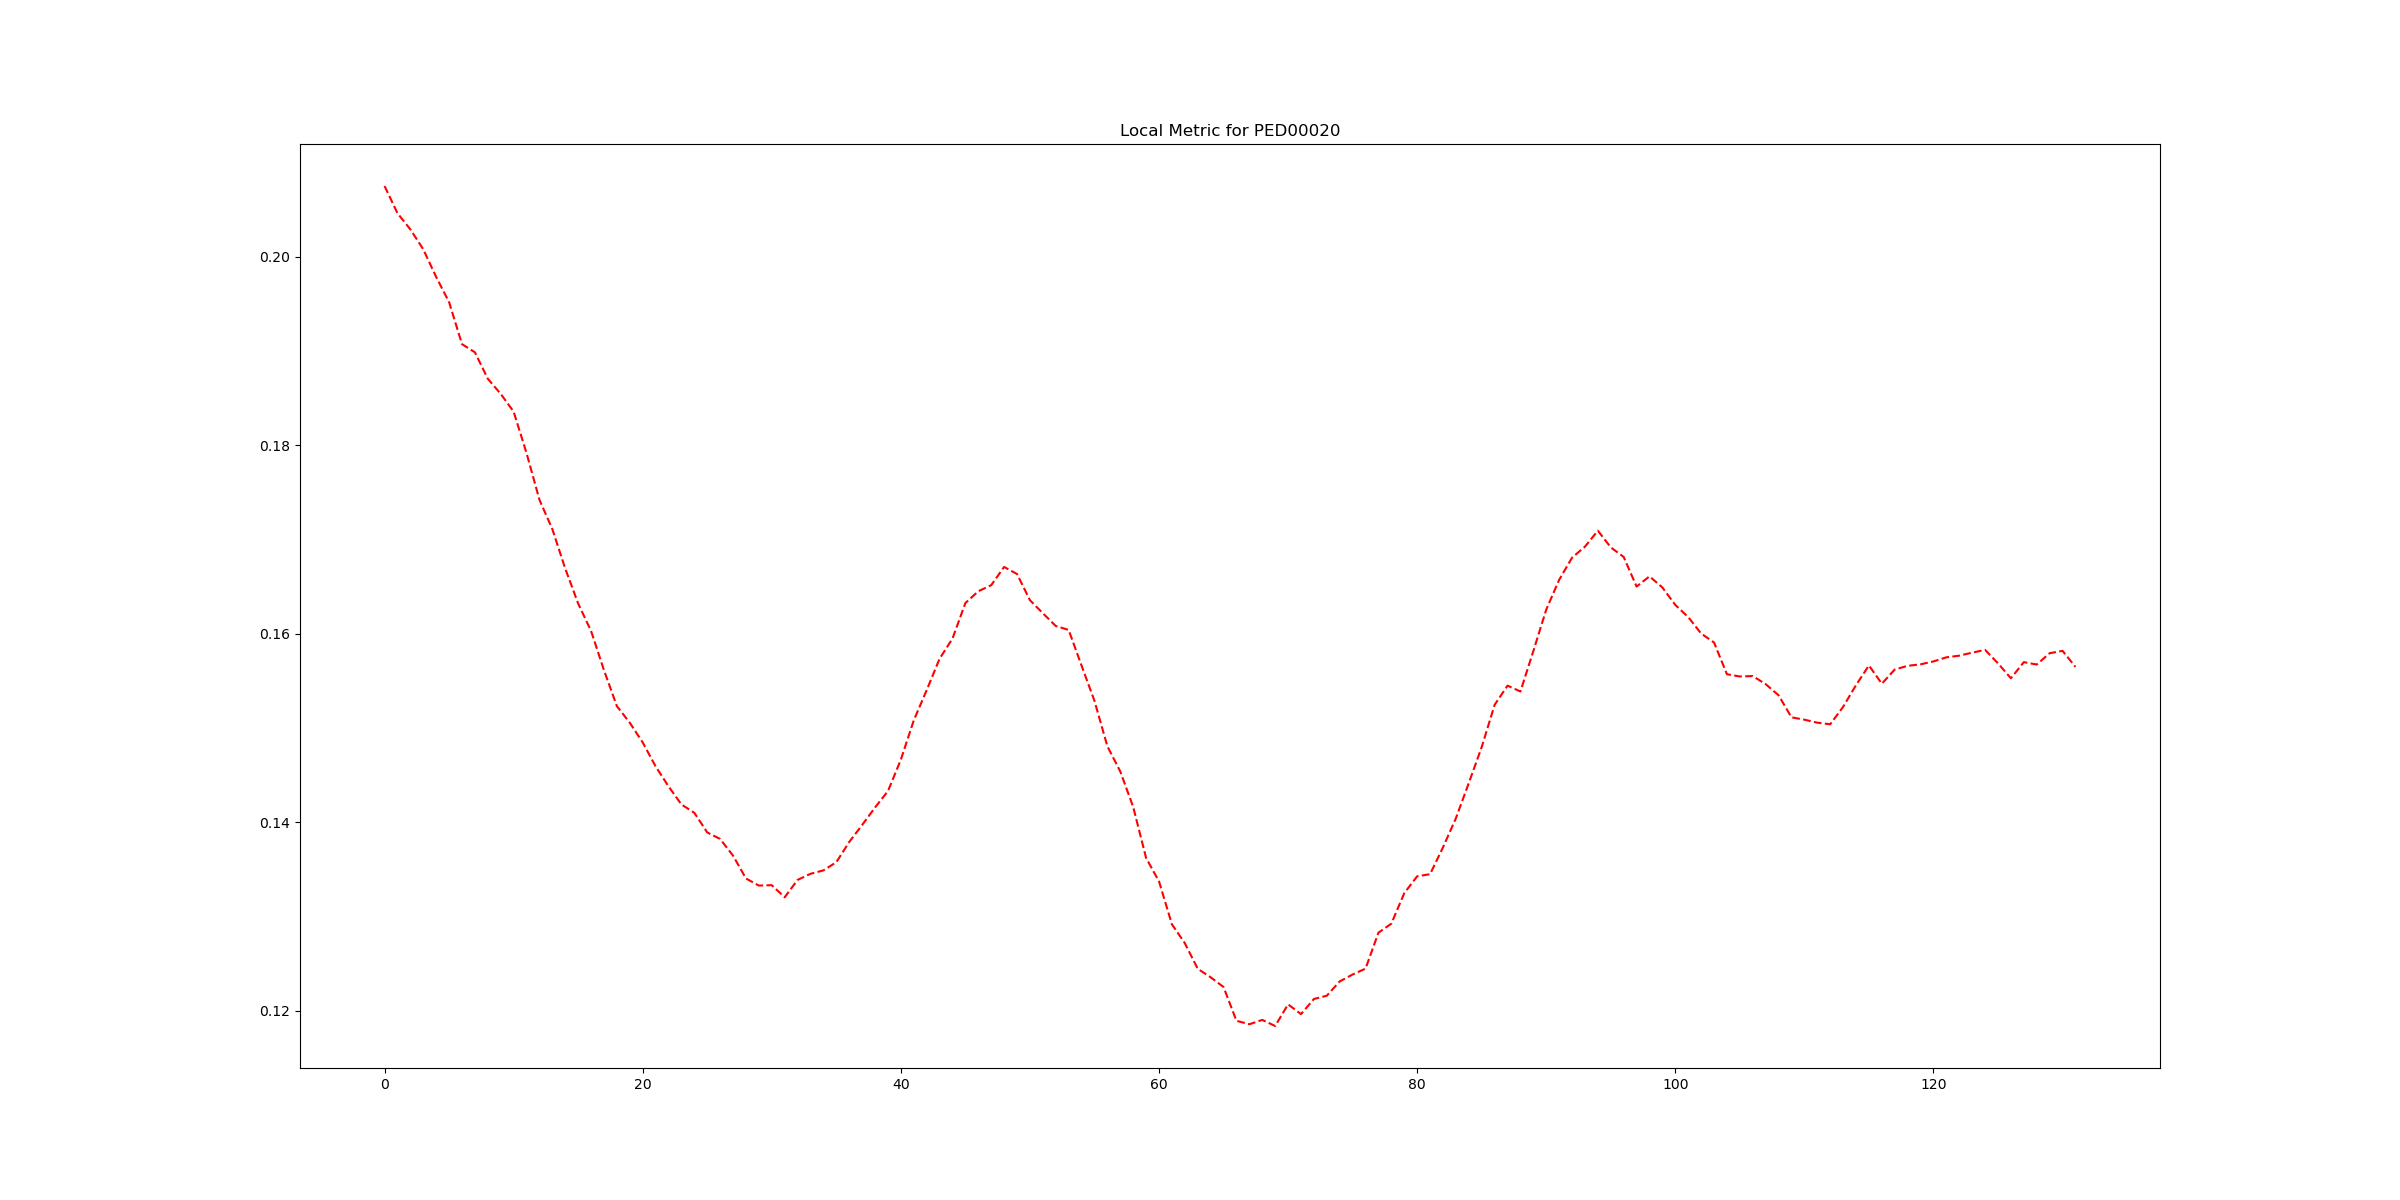
\includegraphics[width=\textwidth]{PED00020_local.png}
		\caption{Plot of local features.}
		\label{plot}
	\end{minipage}	
\end{figure}

In \ref{plot} it is possible to visualize the ensembles' features variation for each residue using the local metric. 

\medskip
Firstly, it is necessary to underline that the graph shows an average value among all the conformations within an ensemble. Therefore, it is not possible to make a precise comparison between the trend of the curve and the variability of the structure in pymol images. 

\medskip
Looking at the graph above and taking into consideration the information extracted from the various comparisons in this project, we can observe that the structure of the measles virus nucleoprotein is quite disordered and there are some points where the variability is greater. 

In particular, we can identify high variability at the beginning of the local graph. Then there are two main minimum points that correspond to stable regions on the structure. At the end the structure variability increases.

This situation can be compared against the pymol color variation. In fact, the region where there is more variability (high value) in the local graph corresponds to a red region in Pymol images, in general. Otherwise, the minimum points are the same blue regions in Pymol.

In conclusion, we can observe that along the ensemble structures there are a few stable points and on average the structure is very messy.

